\section{Clase 32}
\subsection{Modelo de Ising en $D=1$}
Tenemos el siguiente Hamiltoniano
\begin{equation}
  H=\sum_i^N\left(-J\s_i\s_{i+1}-\frac{1}{2}\m B(\s_i+\s_{i+1})\right),\quad \s_{N+1}=1
\end{equation}
Donde $\s_i=\pm 1$ es la orientación del sin $i$ (up o down), $J$ es la constante de acoplamiento entre los spines, $\m$ es el momento magnético y $B$ es el campo magnético externi (en la dirección $+1$).

\begin{figure}[h!]
	\centering
	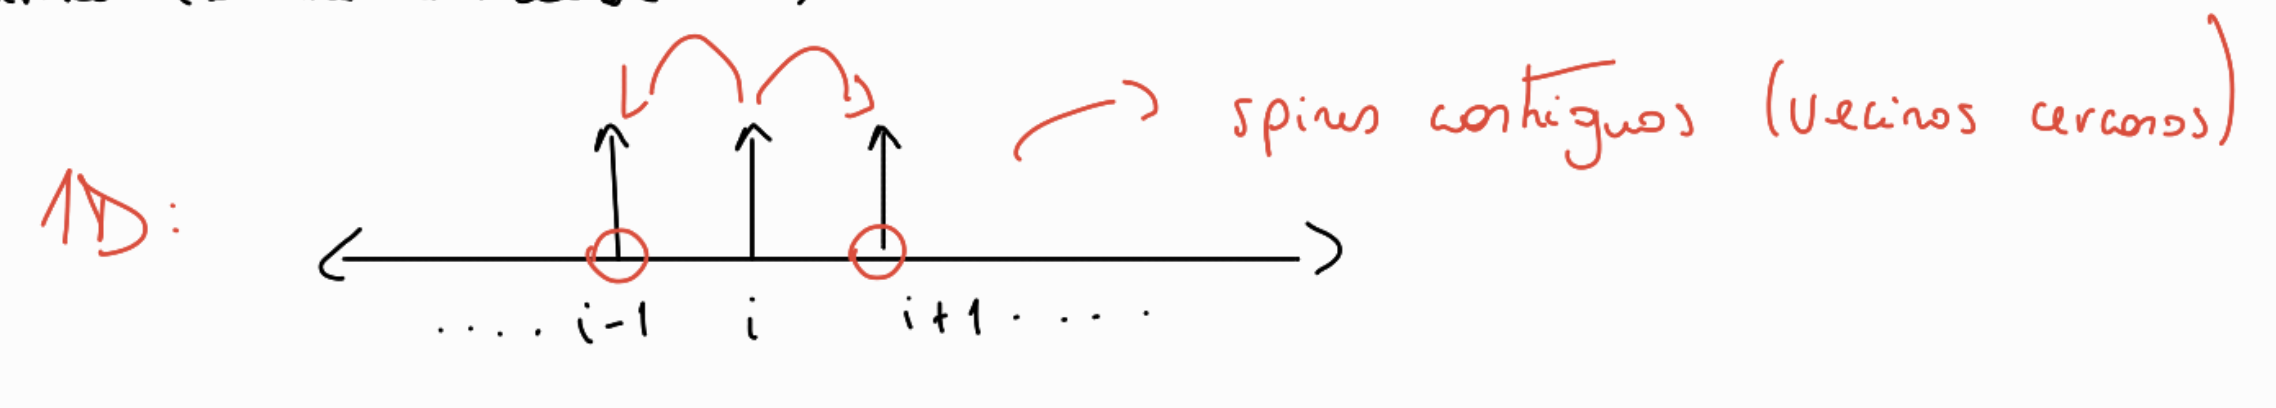
\includegraphics[scale=0.4]{fig/ising}
\end{figure}

La función partición del sistema se puede escribir de la siguiente manera
\begin{equation}
 \boxed{ Z=\sum_{\{\s_i\}_{i=1}^N}e^{-\b H\left(\{\s_i\}\right)}}
\end{equation}

donde $\s_i=\pm 1$ y $\{\s_i\}$ es un conjunto de valores posibles para todos los $N$ spines. Por elemplo, para $N=3$:

\begin{equation}
  \{\s_i \}=\left\{\begin{array}{ll}
  	&1,1,1\\
  	&1,1,-1\\
  	&1,-1,1\\
  	&1,-1,-1\\
  	&-1,1,1\\
  	&-1,1-1\\
  	&-1,-1,1\\
  	&-1,-1,-1
  \end{array}\right.
\end{equation}

Evaluamos el Hamiltoniano para la configuración $1,1,1$,
\begin{align}
  H(\{\s_1,\s_2,\s_3\})&=\sum_{i=1}^3\left(-J\s_i\s_{i+1}-\frac{1}{2}B(\s_i+\s_{i+1})\right)\\
  &=-J\s_1\s_2-J\s_2\s_3-J\s_3\s_1-\m B\s_1-\m B\s_2-\m B\s_3
\end{align}
\begin{equation}
\boxed{  H(\{1,1,1\})=-3J-3\m B}
\end{equation}

\begin{equation}
 H(\{1,-1,1\})=J-\m B
\end{equation}

\begin{ej}
	Escribir la función partición explícita para este sistema con $N=3$.
\end{ej}
En el caso general, la función partición puede reescribirse así,
\begin{equation}
  Z=\sum_{\s_1,...\s_N}\exp[\b (J(\s_1\s_2+\s_2\s_3)+\cdots \s_N\s_1)+\m B(\s_1+\s_2+\cdots \s_N)]
\end{equation}
con $\s_i\in \{+1,-1\}$.

Supongamos el producto de las exponenciales,
\begin{equation}
  Z=\sum_{\s_1,...\s_N}\left(e^{\b(J\s_1\s_2+\m B(\s_1+\s_2))}\right)\left(e^{\b(J\s_2\s_3+\m B(\s_2+\s_3))}\right)+\cdots \left(e^{\b(J\s_N\s_1+\m B(\s_N+\s_1))}\right)
\end{equation}
Lo podemos pensar como una multiplicación de matrices
\begin{equation}\label{32.star}
   Z=\sum_{\s_1,...\s_N}\bra{\s_1}P\ket{\s_2}\bra{\s_2}P\ket{\s_3}\cdots \bra{\s_N}P\ket{\s_1}
\end{equation}
donde
\begin{align}
  P_{i,i+1}&=\exp\left(\b\left[J_{\s_i\s_{i+1}}+\frac{1}{2}\m B(\s_i+\s_{i+1})\right]\right)\\
  &=\mqty(e^{\b(J+\m B)}&&e^{-\b J}\\\\
  e^{-\b J}&& e^{\b (J-\m B)}),\qquad \ket{\s_i}=\ket{\pm 1}
\end{align}

Veamos un ejemplo para $N=3$:
\begin{equation}
  Z=\sum_{\s_1,\s_2,\s_3}\bra{\s_1}P\ket{\s_2}\bra{\s_2}P\ket{\s_3}\bra{\s_3}P\ket{\s_1}
\end{equation}
\begin{align}
  Z&=\bra{1}P\ket{1}\bra{1}P\ket{1}\bra{1}P\ket{1},\qquad \s_1,\s_2,\s_3=1,1,1\\
  &+\bra{1}P\ket{1}\bra{1}P\ket{-1}\bra{-1}P\ket{1},\qquad \s_1,\s_2,\s_3=-1,1,-1\\
  &+\bra{1}P\ket{-1}\bra{-1}P\ket{1}\bra{1}P\ket{1},\qquad \s_1,\s_2,\s_3=-1,-1,1\\
  \vdots 
\end{align}

Entonces 
\begin{equation}
  \mqty(e^{\b(J+\m B)}&&e^{-\b J}\\\\
  e^{-\b J}&& e^{\b (J-\m B)})=\mqty(\bra{1}P\ket{1}&&\bra{-1}P\ket{1}\\\\
  \bra{1}P\ket{-1}&& \bra{-1}P\ket{-1})
\end{equation}
Si imponemos que el último spin deber ser igual al primero es como tener la traza de una matriz,
\begin{equation}
  Z=\sum_{\s_1}\bra{\s_1}P\ket{\s_1}=\Tr (P^N)
\end{equation}
Notar que
\begin{equation}
  \bra{\s_i}P^3\ket{\s_j}=\sum_{\s_1,\s_2,\s_3}\bra{\s_1}P\ket{\s_2}\bra{\s_2}P\ket{\s_3}\bra{\s_3}P\ket{\s_1}
\end{equation}
Usando que
\begin{equation}
  P^3_{i,j}=\sum_{k,l}P_{ik,},P_{kl},P_{lj}
\end{equation}
Por ultimo, como
\begin{equation}
  \Tr M=\sum_i M_{ii}
\end{equation}
Se tiene que
\begin{equation}
  \Tr (P^3)=\sum_{\s_1}\bra{\s_1}P^3\ket{\s_1}
\end{equation}
\begin{equation}
  \Tr(P^3)=\sum \bra{\s_1}P\ket{\s_1}\bra{\s_2}P\ket{\s_3}\bra{\s_3}P\ket{\s_1}
\end{equation}
y luego para $\Tr(P^N)$ se recupera \eqref{32.star}.

Por lo tnato la función partición exacta del sistema, puede escribirse asi,
\begin{align}
  Z&=\Tr(P^N)\\
  &=\Tr(P^NU^\dagger U)\\
  &=\Tr(UP^NU^\dagger)\\
  &=\Tr((UPU^T)^N)
\end{align}
con $U^\dagger U=\mathbb{I}$ y 
\begin{equation}
  P= \mqty(e^{\b(J+\m B)}&&e^{-\b J}\\\\
  e^{-\b J}&& e^{\b (J-\m B)})
\end{equation}

Sea $U$ tal que $UPU^\dagger=P_l=diag(\lambda_+,\lambda_-)$. Entonces se tiene que
\begin{align}
  Z&=\Tr(P^N)\\
  &=\Tr(diag(\lambda_+,\lambda_-)^N)\\
  &=\Tr(diag(\lambda_+^N,\lambda_-^N))\\
  &=\lambda_+^N+\lambda_-^N
\end{align}

Finalmente,
\begin{equation}
\boxed{  Z=\lambda_+^N+\lambda_-^N}
\end{equation}
donde $\lambda_{\pm }$ son los autoestados de $P$.

Para 
\begin{equation}
  P= \mqty(e^{\b(J+\m B)}&&e^{-\b J}\\\\
  e^{-\b J}&& e^{\b (J-\m B)})
\end{equation}
se tiene
\begin{equation}
 \boxed{ \lambda_{\pm }=e^{\b J}\cosh (\b\m B)\pm\sqrt{e^{2\b J}\sinh^2(\b\m B)+e^{-2\b J}}}
\end{equation}

Para encontrar los autoestados de la matriz
\begin{equation}
 M=\mqty(M_{11}&M_{12}\\M_{21}&M_{22})
\end{equation}
debemos considerar $|M-\lambda\mathbb{I}|=0$ y encontrar los $\lambda$ que satisfacen dicha condición (las raices del polinomo caracteristico).

Es decir,
\begin{equation}
  \left|\mqty(M_{11}-\lambda&M_{12}\\M_{21}&M_{22}-\lambda)\right|=(M_{11}-\lambda)(M_{22}-\lambda)-M_{12}M_{21}=0
\end{equation}
\begin{equation}
  \lambda^2-\lambda(M_{11}+M_{22})-M_{12}M_{21}=0
\end{equation}
\begin{equation}
\boxed{  \lambda_{\pm }=\frac{(M_{11}+M_{22})}{2}\pm \sqrt{(M_{11}+M_{22})^2+4M_{12}M_{21}}}
\end{equation}

Notar que, por construcción, $\lambda_+>\lambda_-$. Luego, para $N\to \infty$,
\begin{align}
  \ln(Z)&=\ln(\lambda_+^N+\lambda_-^N)\\
  &=\ln\left(\lambda_+^N\left(1+\left(\frac{\lambda_-}{\lambda_+}\right)^N\right)\right)\\
  &=N\ln(\lambda_+)+\ln\left(1+\left(\frac{\lambda_-}{\lambda_+}\right)^N\right)
\end{align}
Luego,
\begin{equation}
  \lim_{N\to \infty}\left(\frac{\lambda_-}{\lambda_+}\right)^N=0
\end{equation}
porque $(\lambda_-/\lambda_+)<1$. Entonces
\begin{align}
  \lim_{N\to \infty}\ln(Z)&=N\ln(\lambda_+)
\end{align}
Por tanto, para $N$ grande, puede aproximarse:
\begin{equation}
\boxed{  \ln(Z)=N\ln(\lambda_+)}
\end{equation}
con
\begin{equation}
 \boxed{ \lambda_{\pm }=e^{\b J}\cosh (\b\m B)\pm\sqrt{e^{2\b J}\sinh^2(\b\m B)+e^{-2\b J}}}
\end{equation}
Podemos usar la función partición para calcular los valores promedio d los cantidades termodinámicas. Por ejemplo $\ev{\s}$.

\begin{ej}
	En términos de $J,\m,B$ y $T$ ecuentre $\ev{\s }$ en el modelo de Ising en $D=1$.
\end{ej}




































































